

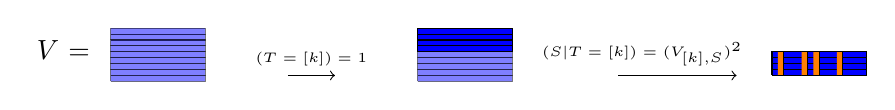
\begin{tikzpicture}[scale = 0.3]

  % draw line and angle
%  \draw 
%     pic [draw,angle radius=4mm,angle eccentricity=1.5, "$\theta$" font=\scriptsize] {angle=v2--v1--v3};

 



 

\draw [fill=blue, opacity=0.5] (-15,3.75) -- (-11,3.75) -- (-11,4) -- (-15,4) -- (-15,3.75);
\draw [fill=blue, opacity=0.5] (-15,3.5) -- (-11,3.5) -- (-11,3.75) -- (-15,3.75) -- (-15,3.5);
\draw [fill=blue, opacity=0.5] (-15,3.25) -- (-11,3.25) -- (-11,3.5) -- (-15,3.5) -- (-15,3.25);
\draw [fill=blue, opacity=0.5] (-15,3) -- (-11,3) -- (-11,3.25) -- (-15,3.25) -- (-15,3);
\draw [fill=blue, opacity=0.5] (-15,2.75) -- (-11,2.75) -- (-11,3) -- (-15,3) -- (-15,2.75); 
\draw [fill=blue, opacity=0.5] (-15,2.5) -- (-11,2.5) -- (-11,2.75) -- (-15,2.75) -- (-15,2.5);
\draw [fill=blue, opacity=0.5] (-15,2.25) -- (-11,2.25) -- (-11,2.5) -- (-15,2.5) -- (-15,2.25);
\draw [fill=blue, opacity=0.5] (-15,2) -- (-11,2) -- (-11,2.25) -- (-15,2.25) -- (-15,2);
\draw [fill=blue, opacity=0.5] (-15,1.75) -- (-11,1.75) -- (-11,2) -- (-15,2) -- (-15,1.75);



\draw [fill=blue, opacity=1] (-2,3.75) -- (2,3.75) -- (2,4) -- (-2,4) -- (-2,3.75);
\draw [fill=blue, opacity=1] (-2,3.5) -- (2,3.5) -- (2,3.75) -- (-2,3.75) -- (-2,3.5);
\draw [fill=blue, opacity=1] (-2,3.25) -- (2,3.25) -- (2,3.5) -- (-2,3.5) -- (-2,3.25);
\draw [fill=blue, opacity=1] (-2,3) -- (2,3) -- (2,3.25) -- (-2,3.25) -- (-2,3);
\draw [fill=blue, opacity=0.5] (-2,2.75) -- (2,2.75) -- (2,3) -- (-2,3) -- (-2,2.75); 
\draw [fill=blue, opacity=0.5] (-2,2.5) -- (2,2.5) -- (2,2.75) -- (-2,2.75) -- (-2,2.5);
\draw [fill=blue, opacity=0.5] (-2,2.25) -- (2,2.25) -- (2,2.5) -- (-2,2.5) -- (-2,2.25);
\draw [fill=blue, opacity=0.5] (-2,2) -- (2,2) -- (2,2.25) -- (-2,2.25) -- (-2,2);
\draw [fill=blue, opacity=0.5] (-2,1.75) -- (2,1.75) -- (2,2) -- (-2,2) -- (-2,1.75);





\draw [fill=blue, opacity=1] (13,2.75) -- (17,2.75) -- (17,3) -- (13,3) -- (13,2.75);
\draw [fill=blue, opacity=1] (13,2.5) -- (17,2.5) -- (17,2.75) -- (13,2.75) -- (13,2.5);
\draw [fill=blue, opacity=1] (13,2.25) -- (17,2.25) -- (17,2.5) -- (13,2.5) -- (13,2.25);
\draw [fill=blue, opacity=1] (13,2) -- (17,2) -- (17,2.25) -- (13,2.25) -- (13,2);


\draw [fill=orange, opacity=1] (13.25,2) -- (13.25,2) -- (13.5,2) -- (13.5,3) -- (13.25,3);
\draw [fill=orange, opacity=1] (14.25,2) -- (14.25,2) -- (14.5,2) -- (14.5,3) -- (14.25,3);
\draw [fill=orange, opacity=1] (14.75,2) -- (14.75,2) -- (15,2) -- (15,3) -- (14.75,3);
\draw [fill=orange, opacity=1] (15.75,2) -- (15.75,2) -- (16,2) -- (16,3) -- (15.75,3);



\draw [->] (-7.5,2) --  (-6.5,2)  node [above] {\tiny $\Prb(T = [k]) = 1$} --  (-5.5,2);

\draw [->] (6.5,2) --  (7.5,2)  node [above] {\tiny $\Prb(S|T = [k]) = \Det (\bm{V}_{[k],S})^{2}$} --  (11.5,2);

\draw  (-17,2.25)  node [above] {$\bm{V}^{\Tran}=$} ;

\end{tikzpicture}
